 \documentclass[landscape, 12pt]{article}

%%%%%%%%%%%%%%%%%%%%%%%%%%%%%%%  Packages  %%%%%%%%%%%%%%%%%%%%%%%%%%%%%%%%%%%%%%
%%%%%%%%%%%%% MATHS %%%%%%%%%%%%%%%%%%%%
\usepackage{amsmath} 
\usepackage{mathtools}
\usepackage{physics}
\usepackage{amssymb}
\usepackage{mathptmx}
%%%%%%%%%%%%%%%%%%%%%%%%%%%%%%%%%%%%%%%%

%%%%%%%%% FIGurES %%%%%%%%%%%%%%%%%%%%%%%%
\usepackage{textcomp}
\usepackage{graphicx}
\usepackage{caption} 
\usepackage{subcaption}
\usepackage{scrextend}
\usepackage{pgfgantt}
\usepackage{rotating}
\usepackage{subcaption}
\usepackage{scrextend}
\usepackage{float}
%\graphicspath{ {figures/} }
%%%%%%%%%%%%%%%%%%%%%%%%%%%%%%%%%%%%%%%%%

%%%%%%%%%%%% LaNgUaGe %%%%%%%%%%%%%%%%%%
\usepackage[latin1]{inputenc}
\usepackage{verbatim}
%%%%%%%%%%%%%%%%

%\usepackage{tikz}
%\usetikzlibrary{shapes,arrows}
%\usetikzlibrary{shapes.geometric, arrows}

% Define block styles
%\tikzstyle{decision} = [diamond, draw, fill=blue!20,text width=4.5em, text badly centered, node distance=3cm, inner sep=0pt]
%\tikzstyle{block} = [rectangle, draw, fill=blue!20, text width=5em, text centered, rounded corners, minimum height=4em]
%\tikzstyle{line} = [draw, -latex']
%\tikzstyle{cloud} = [draw, ellipse,fill=red!20, node distance=3cm,minimum height=2em]

%%%%%%%%%%%%%%%%%% Custom maths shortcuts %%%%%%%%%%%%%%%
\newcommand{\ident}{\[ \mathds{1} \]}

\renewcommand{\vec}[1]{\mathbf{#1}}
\newcommand{\squeezeup}{\vspace{-2.5mm}}
%\DeclarePairedDelimiter\abs{\lvert}{\rvert}%

%\newcommand{\ket}[1]{\left| #1 \right\rangle}
%\newcommand{\bra}[1]{\left\langle #1 \right|}

\usepackage{Qcircuit}
\usepackage{pdflscape}
\usepackage{afterpage}
\usepackage{wrapfig}
\usepackage[a3paper]{geometry}
%%%%%%%%%%%%%%%%%%%%%%%%%%%%%%%%%%%%%%%%%%%%%%%%%%%%%%%%%

\oddsidemargin  0.0in
%\evensidemargin 0.0in
\textwidth      14.25in
%\headheight     0.0in
\topmargin      -0.7in
\textheight=9.5in

%%%%%%%%%%%%%%%%%%%%%%%%%%%%%%%%%%%%%%%%%%% EnD oF pAcKaGeS %%%%%%%%%%%%%%%%%%%%%%%%%%%%%%%%%%%%

\begin{document} %WOOP WOOP!
\begin{comment}
% Title page 

    \title{A practical quantum circuit for the quantum Schur Transform\\ {\Large Project A}}
    \author{Oliver Thomas \\[0.5em] University of Bristol \\ Quantum Engineering CDT}
    \date{\today}
    \maketitle

%\begin{addmargin}[-3em]{-3em}
%%%%%%%%%%%%%%%%%%%%%%%%%%%%%%%%%%%%
\end{comment}

\section{Minimal gate circuit for 2 qubit Schur transform}

\Qcircuit @C=0.6cm @R=0.7cm {
%%%%%%%%%%%%%%%%%% J
%J2
&\lstick{J_2 \ket{0}} &\qw&\qw&\qw&\qw&\qw&\qw&\qw&\qw&\qw&\qw&\qw&\qw&\qw&\qw
&\qw&\qw&\qw&\qw&\qw&\qw&\qw&\qw&\qw
&\qw &\gate{H} &\gate{V} &\qw &\gate{V^{\dag}} &\qw &\gate{V} &\gate{H} &\qw&\qw
&\qw&\qw&\qw  &\rstick{J'_2}
 & \\
%J1
&\lstick{J_1 \ket{0}} &\qw&\qw&\qw&\qw&\qw&\qw&\qw&\qw&\qw&\qw&\qw&\qw&\qw&\qw
&\qw&\qw&\qw&\qw&\qw&\qw&\qw&\qw&\qw
&\targ &\gate{X} &\ctrl{-1} &\targ &\ctrl{-1} &\targ &\qw &\gate{X} &\qw &\targ &\qw
&\qw&\qw &\rstick{J'_1} && \\
%J0
&\lstick{J_0 \ket{0}} &\qw&\qw&\qw&\qw&\qw&\qw&\qw&\qw&\qw&\qw&\qw&\qw&\qw&\qw
&\qw&\qw&\qw&\qw&\qw&\qw&\qw&\qw&\qw 
&\ctrl{-1} &\targ &\qw &\ctrl{-1} &\qw &\ctrl{-1} &\ctrl{-2} &\targ &\qw&\qw &\gate{X}
&\qw&\qw &\rstick{J'_0}
\gategroup{1}{2}{3}{3}{1em}{\{}
\gategroup{1}{36}{3}{38}{1.5em}{\}}
\gategroup{1}{26}{7}{36}{2.5em}{--} 
&  \\
%%%%%%%%%%%%%%%%% M
%M2
&\lstick{m_2 \ket{0}} &\qw&\qw
&\qw &\gate{H} &\gate{V} &\qw &\gate{V^{\dag}} &\qw &\gate{V} &\gate{H} &\qw&\qw&\qw&\qw
&\ctrl{3} &\qw&\qw&\qw&\qw&\qw&\qw&\qw&\qw&\qw&\qw&\qw&\qw&\qw&\qw 
&\qw&\qw&\qw&\qw&\qw&\qw&\qw  &\rstick{m'_2} & \\
%m1
&\lstick{m_1 \ket{0}} &\qw&\qw
&\targ &\gate{X} &\ctrl{-1} &\targ &\ctrl{-1} &\targ &\qw &\gate{X} &\qw &\targ &\qw&\qw&\qw
&\qw&\qw &\ctrlo{1} &\qw &\ctrlo{1} &\ctrlo{2} &\qw&\qw&\qw&\qw&\qw&\qw&\qw&\qw&\qw&\qw&\qw&\qw&\qw&\qw&\qw  &\rstick{m'_1} & \\
%m0
&\lstick{m_0 \ket{0}} &\qw&\qw 
&\ctrl{-1} &\targ &\qw &\ctrl{-1} &\qw &\ctrl{-1} &\qw &\targ &\qw&\qw &\gate{X} &\qw
&\qw&\qw &\ctrlo{1} &\targ &\ctrlo{1} &\targ &\qw&\qw&\qw&\qw&\qw&\qw&\qw
&\qw&\qw&\qw&\qw&\qw&\qw&\qw&\qw&\qw &\rstick{m'_0} 
\gategroup{4}{2}{6}{3}{1em}{\{} 
\gategroup{4}{36}{6}{38}{1.5em}{\}} 
\gategroup{4}{5}{7}{15}{2.5em}{--} 
&&      \\
%%%%%%%%%%%%%%%%%%%%%%%%%%
%Qubit
&\lstick{Spin \ket{s}} &\qw&\qw 
&\qw &\ctrl{-1} &\qw&\qw&\qw&\qw &\ctrl{-3} &\ctrl{-1} &\qw &\ctrl{-2} &\qw&\qw
&\gate{ZX} &\qw &\gate{W} &\qw &\gate{W^{\dag}} &\qw &\gate{W} 
&\qw&\qw&\qw &\ctrl{-4} &\qw&\qw&\qw&\qw&\qw &\ctrl{-4} &\qw &\ctrl{-5} &\qw&\qw&\qw &\rstick{\ket{P}}       
\gategroup{4}{17}{7}{23}{2em}{--} 
%\gategroup{6}{32}{13}{36}{1em}{--}  
%\gategroup{2}{45}{13}{50}{1em}{--}
\\ 
%Labels
&&&&&&&& \mbox{Quantum Adder on m} &&&&&&&&&&& \mbox{Transform spin} &&&&&&&&&&& \mbox{Quantum Adder on J} &&&&&&&&&&&&&&&
}

\vspace{1cm}
%
\begin{wrapfigure}{l}{0.25\textwidth}
\begin{tabular}{ |c c c|c| } 
\hline
 $J_2$ &$J_1$ &$J_0$ &J \\
 \hline
 0 &0 &0 &0 \\ 
 0 &0 &1 &$\frac{1}{2}$ \\ 
 0 &1 &0 &1 \\ 
 0 &1 &1 &$\frac{3}{2}$ \\ 
 \hline 
 1 &0 &0 &-2 \\ 
 1 &0 &1 &-$\frac{3}{2}$ \\ 
 1 &1 &0 &-1 \\ 
 1 &1 &1 &-$\frac{1}{2}$ \\  
 \hline 
\end{tabular}
\quad
\begin{tabular}{ |c c c|c| } 
\hline
 $m_2$ &$m_1$ &$m_0$ &M \\
 \hline
 0 &0 &0 &0 \\ 
 0 &0 &1 &$\frac{1}{2}$ \\ 
 0 &1 &0 &1 \\ 
 0 &1 &1 &$\frac{3}{2}$ \\ 
 \hline 
 1 &0 &0 &-2 \\ 
 1 &0 &1 &-$\frac{3}{2}$ \\ 
 1 &1 &0 &-1 \\ 
 1 &1 &1 &-$\frac{1}{2}$ \\  
 \hline
\end{tabular}
\caption{Tables giving binary Two's complement encoding to spin values of the M and J registers}
\label{fig:encoding}
\quad
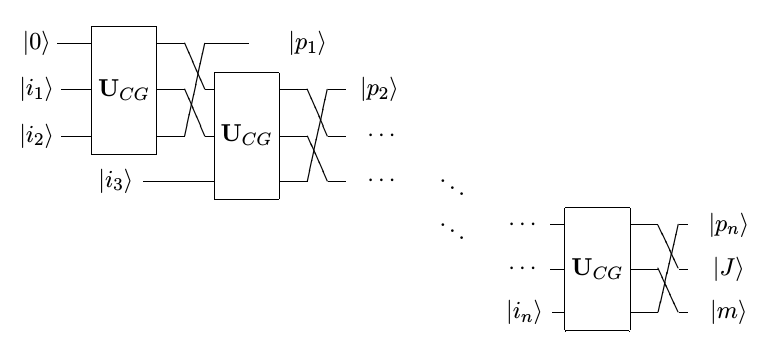
\includegraphics[width=0.25\textwidth]{schurcascade.png}
\caption{Taken from Bacon, Chaung, Harrow (2008) Arxiv /0407082v4}
\vspace{-200pt} 
\end{wrapfigure}

Circuit uses the encoding for $\ket{S} : \ket{0} \mapsto Spin = +\frac{1}{2}, \ket{1} \mapsto Spin = -\frac{1}{2}$ and the same for $\ket{P}$. 

Where $V$ is the phase gate, 
$ V = \begin{bmatrix}
1 & 0 \\
0 & i \\
\end{bmatrix} $
, $V^{\dag}V = I$ and $V^2 = Z$. $V$ is used here to expand the double controlled Toffoli gate into single control gates in the quantum adder subroutine.

The $W$ gate, $W^2 = HX$ with $W^{\dag} = I$, is used to expand the $HX$ gate into single control gates in the spin transform region. 

The circuit checks that if ($m_1$ XNOR $m_0$) AND ($m_0$ XOR $S_0$) and will then change $m_2$. Then $m_1$ is updated using $m_1 = m_0$ XOR $S_0$. $m_0$ is always incremented by 1, if $\ket{S} = \ket{0}$ increment only $m_0$ by 1 corresponding to adding $\frac{1}{2}$ to the $M$ register. $\ket{S} = \ket{1}$ corresponds to subtracting $\frac{1}{2}$ from the $M$ register by adding the string 111 bitwise to $M$. 
 
For the most positive values of $M$ the Identity is performed on the spin corresponding to the strings $M=001 (J=\frac{1}{2}, M' = \frac{1}{2})$ for the first spin and $M=010 (J=1, M'=1) $ for the second coupled in spins. 

The most negative values of $M$ performs $XZ \ket{S}$ corresponding to the strings $M=111 (J=\frac{1}{2}, M'=-\frac{1}{2})$ for the first spin and $M=110 (J=1, M'=-1)$ for the second spin.

If $M=000 (J=0, M'=0)$ do $XH \ket{S}$.  


\newpage
%%%%%%%%%%%%%%%%%%%%%%%%%%%%%%%%%%%%%%%%%%%%%%%%%%%%%%%%%%%%%%%%%%%%%%%%%%%%%%%%
\section{Circuit for the Quantum Schur transform for up to 2 qubits ($\ket{S}$)}
%\begin{landscape}
\Qcircuit @C=0.35cm @R=0.6cm {
%%%%%%%%%%%%%%%%%J-Carry
%j-C2
&\lstick{C_2 \ket{0}} 
&\qw&\qw&\qw&\qw&\qw&\qw&\qw&\qw&\qw&\qw&\qw&\qw&\qw&\qw&\qw&\qw&\qw&\qw&\qw&\qw&\qw&\qw&\qw&\qw&\qw&\qw&\qw&\qw&\qw&\qw&\qw&\qw&\qw&\qw&\qw&\qw&\qw&\qw&\qw&\qw&\qw&\qw&\qw&\qw&\qw&\qw&\qw&\qw&\qw
&\targ&\targ&\targ &\qw
&\ctrl{4} 
&\qw&\qw&\qw &\ctrl{3} &\qw&\qw &\rstick{C_2} &\\
%j-C1
&\lstick{C_1 \ket{0}} 
&\qw&\qw&\qw&\qw&\qw&\qw&\qw&\qw&\qw&\qw&\qw&\qw&\qw&\qw&\qw&\qw&\qw&\qw&\qw&\qw&\qw&\qw&\qw&\qw&\qw&\qw&\qw&\qw&\qw&\qw&\qw&\qw&\qw&\qw&\qw 
&\targ&\targ&\targ &\qw&\qw&\qw&\qw 
&\targ&\targ&\targ &\qw&\qw&\qw&\qw&\qw 
&\ctrl{-1} &\ctrl{-1} &\qw&\qw&\qw&\qw&\qw&\qw&\qw&\qw &\rstick{C_1} &\\
%j-C0
&\lstick{C_0 \ket{0}} \gategroup{1}{2}{3}{3}{1em}{\{}
&\qw&\qw&\qw&\qw&\qw&\qw&\qw&\qw&\qw&\qw&\qw&\qw&\qw&\qw&\qw&\qw&\qw&\qw&\qw&\qw&\qw&\qw&\qw&\qw&\qw&\qw&\qw&\qw&\qw&\qw&\qw&\qw&\qw&\qw&\qw&\qw
&\ctrl{-1} &\ctrl{-1} &\qw &\ctrl{3} &\qw&\qw
&\qw &\ctrl{-1} &\ctrl{-1} &\qw &\ctrl{3} 
&\qw&\qw&\qw&\qw&\qw&\qw&\qw&\qw&\qw&\qw&\qw&\qw&\qw &\rstick{C_0} &\\
%%%%%%%%%%%%%%%%%% J
%J2
&\lstick{J_2 \ket{0}}
&\qw&\qw&\qw&\qw&\qw&\qw&\qw&\qw&\qw&\qw&\qw&\qw&\qw&\qw&\qw&\qw&\qw&\qw&\qw&\qw&\qw&\qw&\qw&\qw&\qw&\qw&\qw&\qw&\qw&\qw&\qw&\qw&\qw&\qw&\qw&\qw&\qw&\qw&\qw&\qw&\qw&\qw&\qw&\qw&\qw&\qw&\qw&\qw&\qw&\qw&\qw&\qw&\qw&\qw&\qw&\qw
&\targ &\targ &\qw&\qw  &\rstick{J'_2} & \\
%J1
&\lstick{J_1 \ket{0}}
&\qw&\qw&\qw&\qw&\qw&\qw&\qw&\qw&\qw&\qw&\qw&\qw&\qw&\qw&\qw&\qw&\qw&\qw&\qw&\qw&\qw&\qw&\qw&\qw&\qw&\qw&\qw&\qw&\qw&\qw&\qw&\qw&\qw&\qw&\qw&\qw&\qw&\qw&\qw&\qw&\qw&\qw&\qw&\qw&\qw&\qw&\qw&\qw&\qw
&\ctrl{-4} &\ctrl{-3} &\qw
&\targ &\targ &\qw&\qw&\qw&\qw&\qw&\qw  &\rstick{J'_1} & \\
%J0
&\lstick{J_0 \ket{0}} \gategroup{4}{2}{6}{3}{1em}{\{}
&\qw&\qw&\qw&\qw&\qw&\qw&\qw&\qw&\qw&\qw&\qw&\qw&\qw&\qw&\qw&\qw&\qw&\qw&\qw&\qw&\qw&\qw&\qw&\qw&\qw 
&\ctrlo{4} &\ctrlo{4} &\qw &\qw&\qw
&\ctrl{5} &\ctrl{4} &\ctrl{4} &\qw&\qw
&\ctrl{-4} &\ctrl{-3} &\qw &\targ &\targ &\qw&\qw 
&\ctrl{-4} &\ctrl{-3} &\ctrl{-3}
&\targ &\targ &\qw&\qw&\qw&\qw&\qw&\qw&\qw&\qw&\qw&\qw&\qw&\qw&\qw
&\rstick{J'_0} \gategroup{4}{60}{6}{61}{1.5em}{\}} &  \\
%%%%%%%%%%%%%%%%%%M-Carry
%m-C2
&\lstick{C_2 \ket{0}} 
&\qw&\qw&\qw&\qw&\qw&\qw&\qw&\qw&\qw&\qw&\qw&\qw&\qw&\qw 
&\targ &\targ &\targ &\qw&\qw&\qw&\qw
&\qw &\ctrl{3} 
&\qw&\qw&\qw&\qw&\qw&\qw&\qw&\qw&\qw&\qw&\qw&\qw&\qw&\qw&\qw&\qw&\qw&\qw&\qw&\qw&\qw&\qw&\qw&\qw&\qw&\qw&\qw&\qw&\qw&\qw&\qw&\qw&\qw&\qw&\qw&\qw&\qw     &\rstick{C_2}    \\
%m-C1
&\lstick{C_1 \ket{0}} 
&\qw &\targ &\targ &\targ &\qw&\qw&\qw 
&\targ &\targ &\targ &\qw&\qw&\qw&\qw
&\qw &\ctrl{-1} &\ctrl{-1} &\qw &\ctrl{3} 
&\qw&\qw&\qw&\qw&\qw&\qw&\qw&\qw&\qw&\qw&\qw&\qw&\qw&\qw&\qw&\qw&\qw&\qw&\qw&\qw&\qw&\qw&\qw&\qw&\qw&\qw&\qw&\qw&\qw&\qw&\qw&\qw&\qw&\qw&\qw&\qw&\qw&\qw&\qw&\qw&\qw &\rstick{C_1}           \\
%m-C0
&\lstick{C_0 \ket{0}} \gategroup{7}{2}{9}{3}{1em}{\{}
&\qw&\qw &\ctrl{-1} &\ctrl{-1} &\qw &\ctrl{3} &\qw&\qw 
&\ctrl{-1} &\ctrl{-1} &\qw &\ctrl{3} &\qw
&\qw&\qw&\qw&\qw&\qw&\qw&\qw&\qw&\qw&\qw&\qw&\qw&\qw&\qw&\qw&\qw&\qw&\qw&\qw&\qw&\qw&\qw&\qw&\qw&\qw&\qw&\qw&\qw&\qw&\qw&\qw&\qw&\qw&\qw&\qw&\qw&\qw&\qw&\qw&\qw&\qw&\qw&\qw&\qw&\qw&\qw&\qw  &\rstick{C_0}     \\
%%%%%%%%%%%%%%%%% M
%M2
&\lstick{m_2 \ket{0}}
&\qw&\qw&\qw&\qw&\qw&\qw&\qw&\qw&\qw&\qw&\qw&\qw&\qw&\qw&\qw&\qw&\qw&\qw&\qw&\qw&\qw 
&\targ &\targ &\qw&\qw
&\ctrlo{3} &\ctrl{3} &\qw&\qw&\qw 
&\qw &\ctrlo{1} &\ctrl{3} 
&\qw&\qw&\qw&\qw&\qw&\qw&\qw&\qw&\qw&\qw&\qw&\qw&\qw&\qw&\qw&\qw&\qw&\qw&\qw&\qw&\qw&\qw&\qw&\qw&\qw&\qw&\qw &\rstick{m'_2}   &    \\
%m1
&\lstick{m_1 \ket{0}}
&\qw&\qw&\qw&\qw&\qw&\qw
&\qw&\qw&\qw&\qw&\qw &\qw&\qw&\qw
&\ctrl{-4} &\ctrl{-3} &\qw &\targ &\targ
&\qw&\qw&\qw&\qw&\qw&\qw&\qw &\qw&\qw&\qw&\qw
&\ctrl{2} &\ctrlo{2} &\qw&\qw&\qw&\qw
&\qw&\qw&\qw&\qw&\qw&\qw&\qw&\qw&\qw&\qw&\qw&\qw&\qw&\qw&\qw&\qw&\qw&\qw&\qw&\qw&\qw&\qw&\qw&\qw  &\rstick{m'_1}   &      \\
%m0
&\lstick{m_0 \ket{0}} \gategroup{10}{2}{12}{3}{1em}{\{} \gategroup{7}{10}{13}{15}{1em}{--} &\qw
&\ctrl{-4} &\ctrl{-3} &\qw &\targ &\targ &\qw
&\ctrl{-4} &\ctrl{-3} &\qw &\targ &\targ &\qw&\qw
&\qw&\qw&\qw&\qw&\qw&\qw&\qw&\qw&\qw&\qw&\qw&\qw&\qw&\qw&\qw&\qw&\qw
&\qw &\qw&\qw&\qw&\qw&\qw&\qw&\qw&\qw&\qw&\qw&\qw
&\qw&\qw&\qw&\qw&\qw&\qw&\qw&\qw&\qw&\qw&\qw&\qw&\qw&\qw&\qw&\qw&\qw &\rstick{m'_0} \gategroup{10}{60}{12}{61}{1.5em}{\}} &&      \\
%%%%%%%%%%%%%%%%%%%%%%%%%%
%Qubit
&\lstick{Spin \ket{s}} &\qw 
&\ctrlo{-1} &\qw &\ctrlo{-4} &\ctrlo{-1} &\qw&\qw
&\ctrl{-1} &\qw &\ctrl{-4} &\ctrl{-1} &\qw&\qw&\qw 
&\ctrl{-2} &\qw &\ctrl{-5} &\ctrl{-2} &\qw&\qw&\qw 
&\ctrl{-3} &\qw&\qw&\qw &\gate{I} &\gate{ZX} \gategroup{6}{27}{13}{30}{1em}{--} 
&\qw&\qw&\qw &\gate{I} &\gate{HX} &\gate{ZX} \gategroup{6}{32}{13}{36}{1em}{--} &\qw&\qw 
&\ctrlo{-7} &\qw &\ctrlo{-10} &\ctrlo{-7} &\qw&\qw&\qw 
&\ctrl{-7} &\qw &\ctrl{-7} &\ctrl{-7} &\qw&\qw&\qw  \gategroup{2}{45}{13}{50}{1em}{--} 
&\ctrl{-8} &\qw &\ctrl{-11} &\ctrl{-8} &\qw&\qw&\qw
&\ctrl{-9} \qw&\qw&\qw&\qw  &\rstick{\ket{P}}         \\ 
%Labels
&&&&&&&&&&& \mbox{Quantum Adder} &&&&&&&&&&&&&&&& \mbox{$1^{st}$ Spin} &&&&&& \mbox{$2^{nd}$ Spin} &&&&&&&&&&&&& \mbox{Quantum Adder} &&&&&&&&&&&&&&&&&&&&&&&&&&&&&&&&&
}
\vspace{0.5cm}
%
\begin{wrapfigure}{L}{0.22\textwidth}
\begin{tabular}{ |c c c|c| } 
\hline
 $J_2$ &$J_1$ &$J_0$ &J \\
 \hline
 0 &0 &0 &0 \\ 
 0 &0 &1 &$\frac{1}{2}$ \\ 
 0 &1 &0 &1 \\ 
 0 &1 &1 &$\frac{3}{2}$ \\ 
 \hline 
 1 &0 &0 &-2 \\ 
 1 &0 &1 &-$\frac{3}{2}$ \\ 
 1 &1 &0 &-1 \\ 
 1 &1 &1 &-$\frac{1}{2}$ \\  
 \hline 
\end{tabular}
\quad
\begin{tabular}{|c c c|c|} 
\hline
 $m_2$ &$m_1$ &$m_0$ &M \\
 \hline
 0 &0 &0 &0 \\ 
 0 &0 &1 &$\frac{1}{2}$ \\ 
 0 &1 &0 &1 \\ 
 0 &1 &1 &$\frac{3}{2}$ \\ 
 \hline 
 1 &0 &0 &-2 \\ 
 1 &0 &1 &-$\frac{3}{2}$ \\ 
 1 &1 &0 &-1 \\ 
 1 &1 &1 &-$\frac{1}{2}$ \\  
 \hline
\end{tabular}
\caption{Tables giving binary Two's complement encoding to spin values of the M and J registers}
\label{fig:subim1}
\end{wrapfigure}

Circuit uses the encoding for $\ket{S} : \ket{0} \mapsto Spin = +\frac{1}{2}, \ket{1} \mapsto Spin = -\frac{1}{2}$ and the same for $\ket{P}$. 

The circuit adds the value of the spin to be added, $\ket{S}$, to the M register to calculate the M' register value. This is done by implementing the quantum reversible equivalent to the digital full adder. 

The case where $\ket{S} = \ket{0}$ means the spin is $+\frac{1}{2}$ so to add $\frac{1}{2}$ to M one is added to the $m_0$ bit. The very first Quantum Adder (QAdd) uses Toffoli gates controlled on $\ket{0}$ on $\ket{s}$ (denoted by the white control circle) with the current $m_0$ value and $C_0$ (an ancilla carry) so that in the case $m_0 = 1$ and we try and add 1 to it, $m_0$ goes to 0 and $m_1$ is increased using the carry as $001+1=010$. The rest of the QAdd stages then just check the carry of the previous qubit to complete to M $+ \frac{1}{2}$ addition as $\ket{S} = \ket{0}$ does not trigger any of the rest of the control gates.

The case where $\ket{S} = \ket{1}$ means the spin is $-\frac{1}{2}$ we do M $-\frac{1}{2}$ which is done by adding the binary string for $-\frac{1}{2}$ which is the all 1's string, 111. This time the very first Quantum Adder does not trigger and $\ket{s}$ is then added to all of the bits of M using C-NOT gates with carries to check for overflow. 

The Unitary is then performed on $\ket{S}$ depending on the values of the newly calculated M' and J registers. The Identity is shown in the circuit for completeness on all the J and M' values. The J register is then updated to J' by adding the value of $\ket{P}$ to J using the QAdd sequence of gates.

To add the second qubit in the values of J' and M' are passed in as the initial register values. It is easy to extend this to many qubits being streamed in one at a time by carefully conditioning the controls on the unitaries, I think in the general case you need at most N controls for coupling up to N qubits in one at a time. The circuit written here has redundancy in the Identity and ZX gates appearing twice. 




\begin{comment}
\Qcircuit @C=0.4cm @R=1.0cm {
%%%%%%%%%%%%%%%%%J-Carry
%j-C1
&\lstick{C_1 \ket{0}} &\qw&\qw&\qw&\qw&\qw&\qw&\qw&\qw&\qw&\qw&\qw&\qw&\qw&\qw&\qw&\qw&\qw&\qw&\qw&\qw&\qw&\qw&\qw&\qw&\qw&\qw &\targ&\targ&\targ &\qw&\qw &\targ&\targ&\targ &\qw&\qw&\qw&\qw &\ctrl{2} &\qw&\qw&\qw     \\
%j-C0
&\lstick{C_0 \ket{0}} \gategroup{1}{2}{2}{3}{1em}{\{} &\qw&\qw&\qw&\qw&\qw&\qw&\qw&\qw&\qw&\qw&\qw&\qw&\qw&\qw&\qw&\qw&\qw&\qw&\qw&\qw&\qw&\qw&\qw&\qw&\qw&\qw&\qw &\ctrl{-1} &\ctrl{-1} &\qw &\ctrl{2} &\qw &\ctrl{-1} &\ctrl{-1} &\qw &\ctrl{2} &\qw&\qw&\qw&\qw&\qw&\qw  \\
%%%%%%%%%%%%%%%%%% J
%J1
&\lstick{J_1 \ket{0}} &\qw&\qw&\qw&\qw&\qw&\qw&\qw&\qw&\qw&\qw&\qw&\qw&\qw&\qw&\qw&\qw&\qw&\qw&\qw&\qw&\qw&\qw&\qw&\qw&\qw&\qw&\qw&\qw&\qw&\qw&\qw&\qw&\qw&\qw&\qw&\qw&\qw &\targ &\targ &\qw&\qw&\qw      \\
%J0
&\lstick{J_0 \ket{0}} \gategroup{3}{2}{4}{3}{1em}{\{} &\qw&\qw&\qw&\qw&\qw&\qw&\qw&\qw&\qw&\qw&\qw&\qw&\qw&\qw&\qw&\qw&\qw&\qw&\qw &\ctrlo{4} &\ctrlo{4} &\qw &\ctrl{4} &\qw &\ctrl{4} &\qw &\ctrl{-3} &\ctrl{-2} &\qw &\targ &\targ &\ctrl{-3} &\ctrl{-2} &\ctrl{-2} &\targ &\targ &\qw&\qw&\qw&\qw&\qw&\qw   \\
%%%%%%%%%%%%%%%%%%M-Carry
%m-C2
&\lstick{C_2 \ket{0}} &\qw&\qw&\qw&\qw&\qw&\qw&\qw&\qw&\qw&\qw&\qw &\targ &\targ &\targ &\qw&\qw&\qw &\ctrl{3} &\qw&\qw&\qw&\qw&\qw&\qw&\qw&\qw&\qw&\qw&\qw&\qw&\qw&\qw&\qw&\qw&\qw&\qw&\qw&\qw&\qw&\qw&\qw&\qw         \\
%m-C1
&\lstick{C_1 \ket{0}} &\qw &\targ &\targ &\targ &\qw &\qw &\targ &\targ &\targ &\qw&\qw&\qw &\ctrl{-1} &\ctrl{-1} &\qw &\ctrl{3} &\qw&\qw&\qw&\qw&\qw&\qw&\qw&\qw&\qw&\qw&\qw&\qw&\qw&\qw&\qw&\qw&\qw&\qw&\qw&\qw&\qw&\qw&\qw&\qw&\qw&\qw            \\
%m-C0
&\lstick{C_0 \ket{0}} \gategroup{5}{2}{7}{3}{1em}{\{} &\qw&\qw &\ctrl{-1} &\ctrl{-1} &\qw &\ctrl{3} &\qw &\ctrl{-1} &\ctrl{-1} &\qw &\ctrl{3} &\qw&\qw&\qw&\qw&\qw&\qw&\qw&\qw&\qw&\qw&\qw&\qw&\qw&\qw&\qw&\qw&\qw&\qw&\qw&\qw&\qw&\qw&\qw&\qw&\qw&\qw&\qw&\qw&\qw&\qw&\qw       \\
%%%%%%%%%%%%%%%%% M
%M2
&\lstick{m_2 \ket{0}} &\qw&\qw&\qw&\qw&\qw&\qw&\qw&\qw&\qw&\qw&\qw&\qw&\qw&\qw&\qw&\qw &\targ &\targ &\qw &\ctrlo{3} &\ctrl{3} &\qw &\ctrlo{1} &\ctrlo{1} &\ctrl{3} &\qw&\qw&\qw&\qw&\qw&\qw&\qw&\qw&\qw&\qw&\qw&\qw&\qw&\qw&\qw&\qw&\qw        \\
%m1
&\lstick{m_1 \ket{0}} &\qw&\qw&\qw&\qw&\qw&\qw&\qw&\qw&\qw&\qw&\qw &\ctrl{-4} &\ctrl{-3} &\qw &\targ &\targ &\qw&\qw&\qw&\qw&\qw&\qw &\ctrl{2} &\ctrlo{1} &\qw&\qw&\qw&\qw&\qw&\qw&\qw&\qw&\qw&\qw&\qw&\qw&\qw&\qw&\qw&\qw&\qw&\qw           \\
%m0
&\lstick{m_0 \ket{0}} \gategroup{8}{2}{10}{3}{1em}{\{} \gategroup{6}{9}{11}{13}{1em}{--} &\qw &\ctrl{-4} &\ctrl{-3} &\qw &\targ &\targ &\ctrl{-4} &\ctrl{-3} &\qw &\targ &\targ &\qw&\qw&\qw&\qw&\qw&\qw&\qw&\qw&\qw&\qw&\qw&\qw &\ctrlo{1} &\qw&\qw&\qw&\qw&\qw&\qw&\qw&\qw&\qw&\qw&\qw&\qw&\qw&\qw&\qw&\qw&\qw&\qw        \\
%%%%%%%%%%%%%%%%%%%%%%%%%%
%Qubit
&\lstick{\ket{s} \ket{0}} &\qw &\ctrlo{-1} &\qw &\ctrlo{-4} &\ctrlo{-1} &\qw &\ctrl{-1} &\qw &\ctrl{-4} &\ctrl{-1} &\qw &\ctrl{-2} &\qw &\ctrl{-5} &\ctrl{-2} &\qw &\ctrl{-3} &\qw&\qw &\gate{I} &\gate{ZX} \gategroup{4}{22}{11}{23}{1em}{--} &\qw &\gate{I} &\gate{HX} &\gate{ZX} \gategroup{4}{25}{11}{27}{1em}{--} &\qw &\ctrlo{-7} &\qw &\ctrlo{-9} &\ctrlo{-7} &\qw &\ctrl{-7} &\qw &\ctrl{-7} &\ctrl{-7} &\qw&\qw &\ctrl{-8} &\qw&\qw&\qw&\qw           \\ 
%Labels
&&&&&&&&&& \mbox{Quantum Adder} &&&&&&&&&&&& \mbox{$1^{st}$ Spin} &&& \mbox{$2^{nd}$ Spin}
}
\end{comment}

%%%%%%%%%%%%%%
%\end{addmargin}
\end{document}
